\documentclass[12pt]{article}
\usepackage[utf8]{inputenc}
\usepackage{parskip}
\usepackage{url}
\usepackage{graphicx}
\usepackage{float}
\usepackage{microtype} % Slightly tweak font spacing for aesthetics
\usepackage{hyperref}

\usepackage{menukeys} % Used to provide graphical key combinations, menu items and file paths.

% Start document here

\begin{document}

% Cover page
\begin{center}

\includegraphics[scale=0.7]{images/logo.jpg}
\end{center}

\renewcommand\thepage{}

% Title page
\begin{titlepage}
\begin{centering}
\huge{Murcs' User Guide}

\vspace{1cm}

\large{Last updated \\ \today}

\vfill

\large{Created by Suspiciously Willing Software \textregistered}

\end{centering}
\thispagestyle{empty}
\end{titlepage}



% Copyright page

Copyright \textcopyright 2015 Daniel van Wichen, Dion Woolley, Haydon Baddock, James Fairbairn, Jay Harris, Matthew Knox

Permission is hereby granted, free of charge, to any person obtaining a copy
of this software and associated documentation files \(the "Software"\), to deal
in the Software without restriction, including without limitation the rights
to use, copy, modify, merge, publish, distribute, sublicense, and/or sell
copies of the Software, and to permit persons to whom the Software is
furnished to do so, subject to the following conditions:

The above copyright notice and this permission notice shall be included in
all copies or substantial portions of the Software.

THE SOFTWARE IS PROVIDED "AS IS", WITHOUT WARRANTY OF ANY KIND, EXPRESS OR
IMPLIED, INCLUDING BUT NOT LIMITED TO THE WARRANTIES OF MERCHANTABILITY,
FITNESS FOR A PARTICULAR PURPOSE AND NONINFRINGEMENT. IN NO EVENT SHALL THE
AUTHORS OR COPYRIGHT HOLDERS BE LIABLE FOR ANY CLAIM, DAMAGES OR OTHER
LIABILITY, WHETHER IN AN ACTION OF CONTRACT, TORT OR OTHERWISE, ARISING FROM,
OUT OF OR IN CONNECTION WITH THE SOFTWARE OR THE USE OR OTHER DEALINGS IN
THE SOFTWARE.

\thispagestyle{empty}

% A preface, containing details of related documents and information on how to navigate the user guide
\section{Preface}

% A contents page
\tableofcontents

% A guide on how to use at least the main functions of the system
\section{Functionality}

% \begin{figure}[H]
% \centering
% 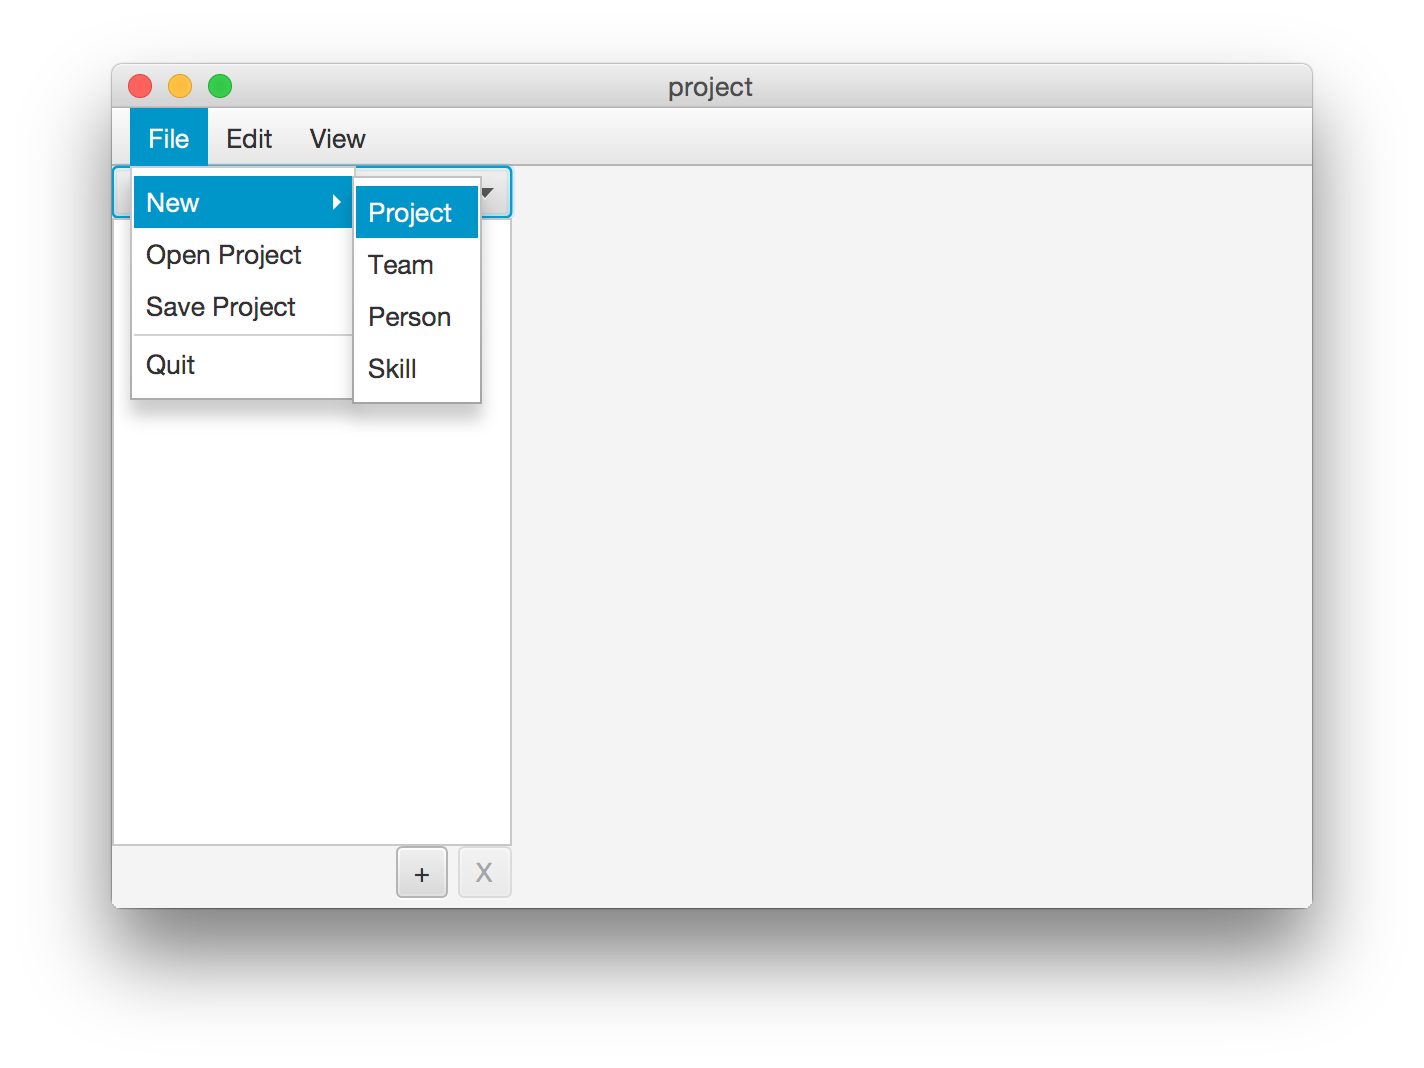
\includegraphics[width=\textwidth]{images/screenshots/screenshot1.png}
% \caption{Creation of new project}
% \label{fig:new_project}
% \end{figure}

\begin{figure}[H]
\centering
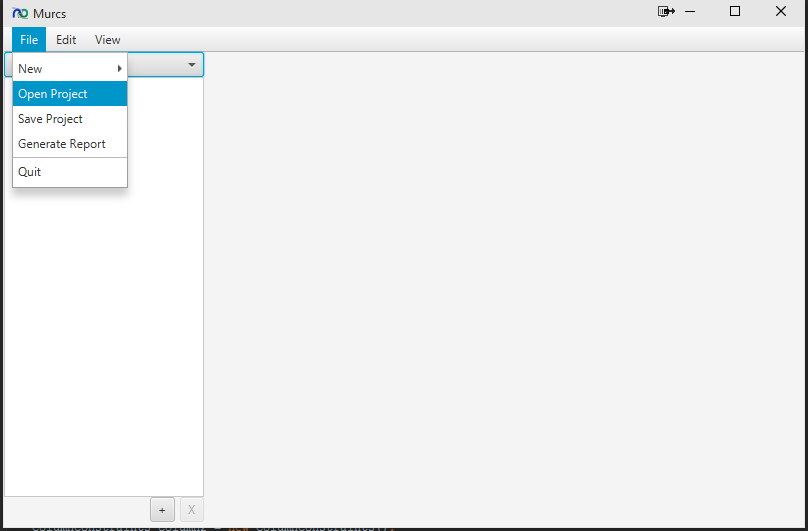
\includegraphics[width=\textwidth]{images/screenshots/openProject.png}
\caption{Open saved project}
\label{fig:open_project}
\end{figure}

\begin{figure}[H]
\centering
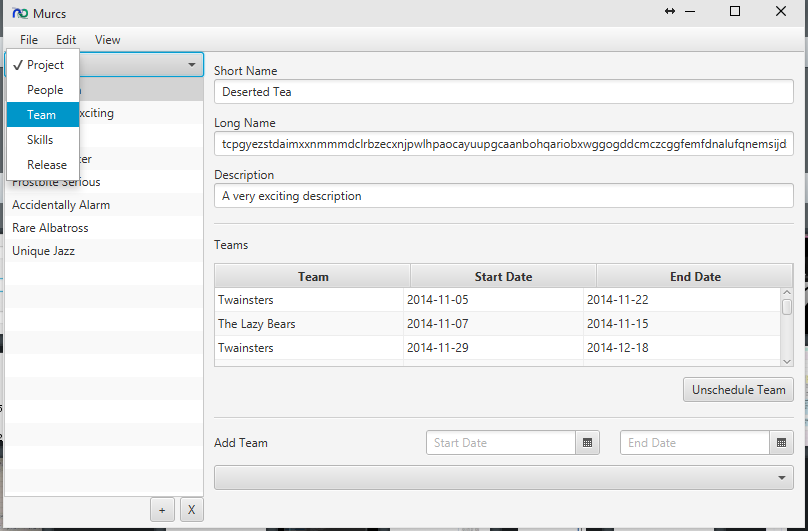
\includegraphics[width=\textwidth]{images/screenshots/changeListView.png}
\caption{Changing views}
\label{fig:change_view}
\end{figure}

% \begin{figure}[H]
% \centering
% 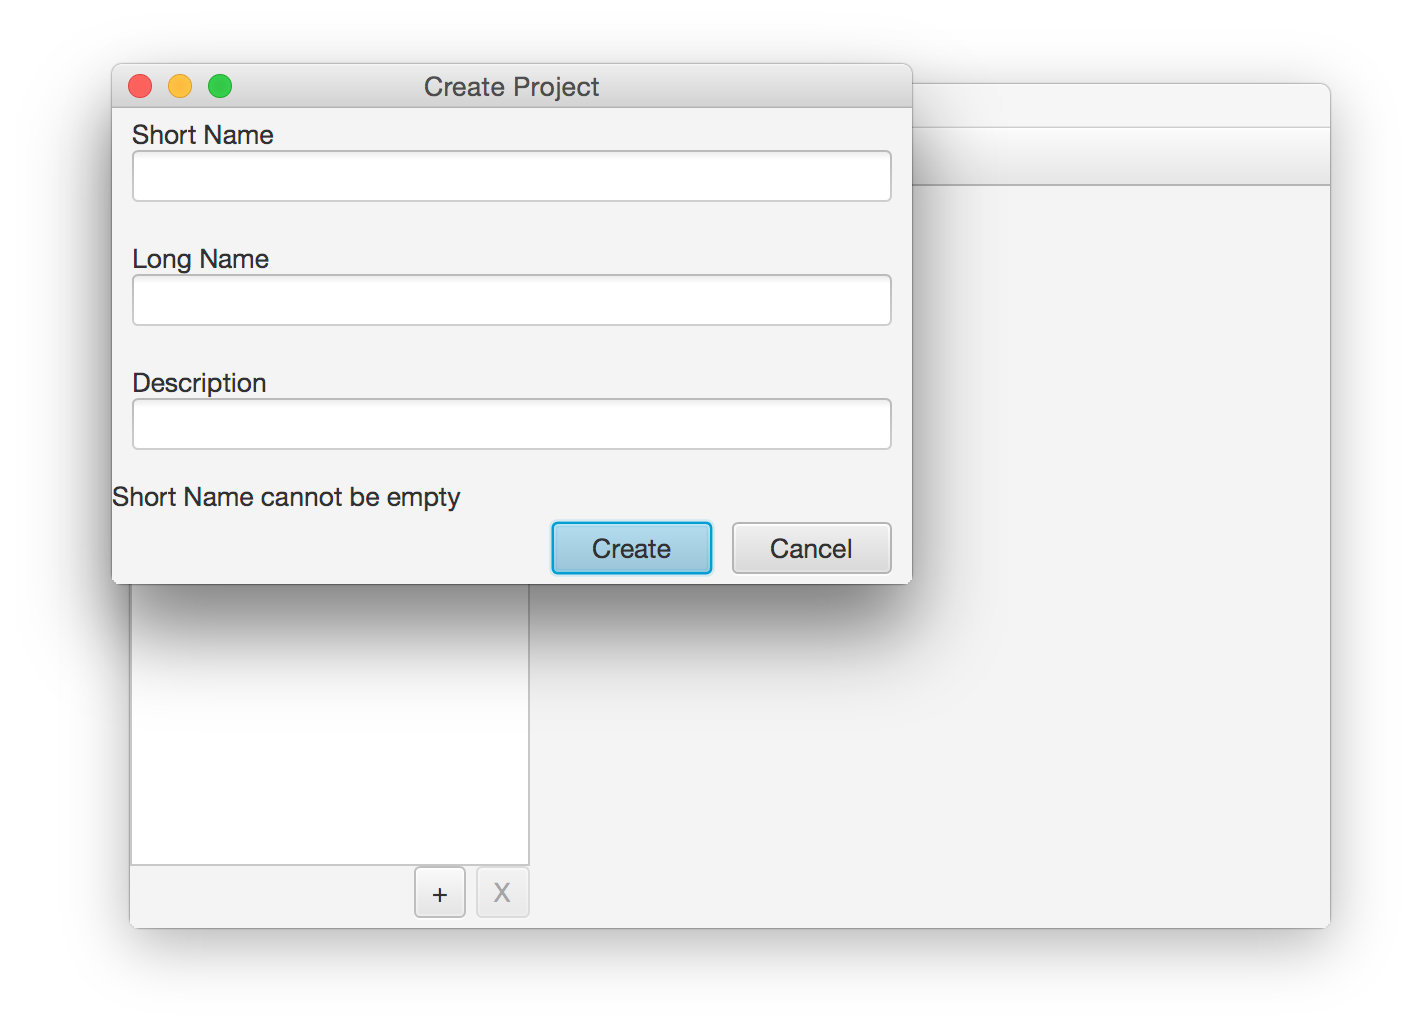
\includegraphics[width=\textwidth]{images/screenshots/screenshot4.png}
% \caption{New project form completion}
% \label{fig:new_project_form}
% \end{figure}

% A guide for deleting elements
\section{Element Deletion}

Elements can easily be deleted using the delete button found in the toolbar. You can also press delete with the item you want to delete selected. Following is a simple walk through for deleting an element.

First, choose the type of the element you wish to delete. This can be either Projects, Teams, People, Skills, Releases, Backlogs, Stories or Sprints and select it in the Display Choice Picker (circled below).

\begin{figure}[H]
\centering
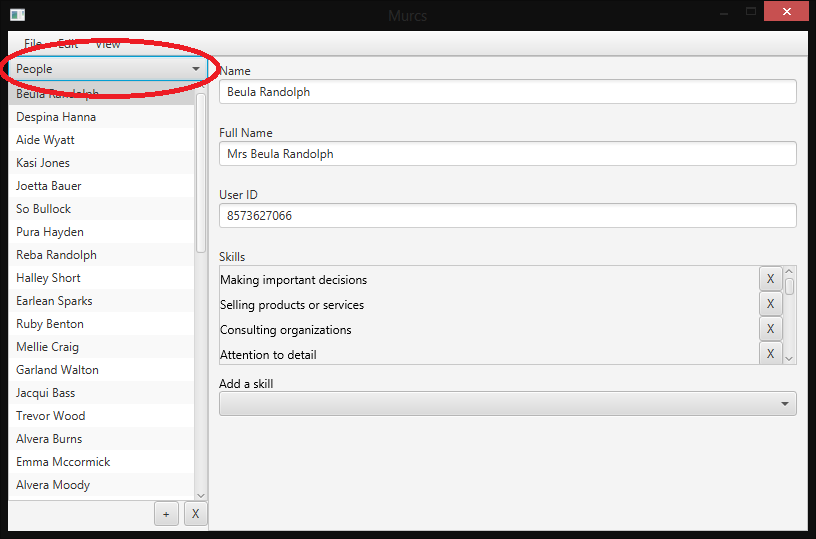
\includegraphics[width=\textwidth]{images/screenshots/deletion1.PNG}
\caption{The Display Choice Picker}
\label{fig:new_project}
\end{figure}

In our case, we've chosen to delete a person named Dion Vader. The next step is to select this person and press the delete button (circled below).

\begin{figure}[H]
\centering
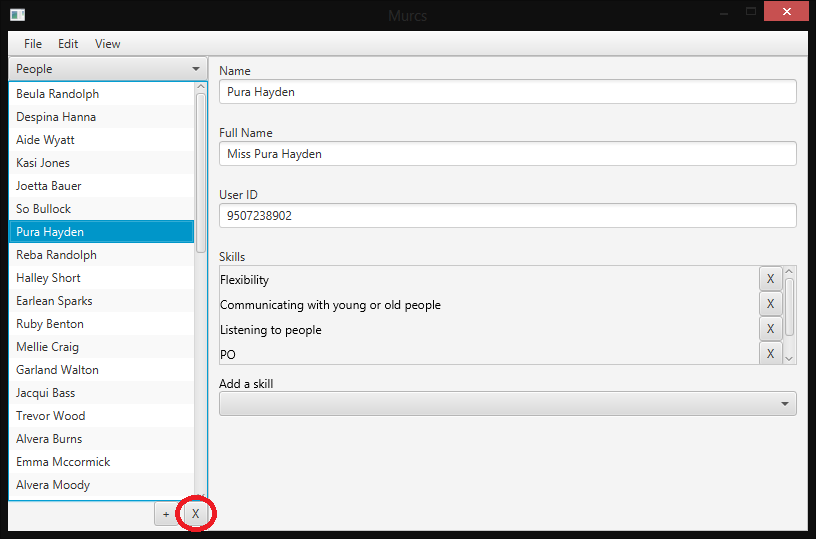
\includegraphics[width=\textwidth]{images/screenshots/deletion2.PNG}
\caption{The Delete Button}
\label{fig:new_project}
\end{figure}

The final step is to confirmation. You will be a presented with a message asking you if you are really sure you want to go through with a deletion along with a list of places that the element you are deleting is used. Press the 'Yes' button (circled) to go through with the deletion. If you've changed your mind you can click the 'No' button. 

\begin{figure}[H]
\centering
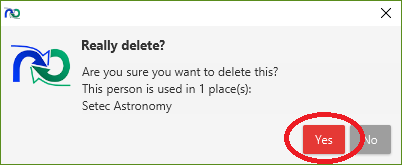
\includegraphics[width=\textwidth]{images/screenshots/deletion3.PNG}
\caption{The Confirmation Dialog. It seems Dion is part of a team named 'Setec Astronomy'}
\label{fig:new_project}
\end{figure}

Deleting Dion also removes him from anywhere else he may be used, so be careful!

If you've deleted something by mistake, don't worry! Deletions can be undone. Phew.

% A troubleshooting section detailing possible errors or problems that may occur, along with how to fix them
\section{Troubleshooting}

Try turning it on and off again. If that fails contact the developers at s301g1@cosc.canterbury.ac.nz

% A FAQ (Frequently Asked Questions)
\section{Frequently Asked Questions}

\newcommand{\faqentry}[2]{\textbf{Q. #1}\\  \textbf{A.} \textit{#2}\vspace{0.5cm}}


\faqentry{How do I make it work?}{Run it from the jar or compile it from the source code}

\faqentry{Can I make it generate random information to use as a starting base?}{Yes. Simply add the argument debug (with optional low, medium high afterwards) when you run the jar and it will automatically generate some information for you to use. This may be a bit more technical than most people will want. It is also not supported by us so if it goes wrong you can't blame us as you've been warned.}

\faqentry{What happens with my old projects?}{Currently they will not be loaded at all and a dialog will appear informing you to open it with the same version of the application that you created it with. We are working towards having support for all old version of .project files.}

\faqentry{
Are there any bugs?
}
{
Yes. The current bugs that we know of include: \newline \begin{itemize}
  \item People can not be unassigned from roles within teams, they can only be replaced.
  \item When a creation form detects an error in input it isn't always very obvious as sometimes it is hidden.
  \item When creating a project if a invalid work allocation is added, the project can not be created.
  \item Status reports are not pretty printed correctly.
  \item (Minor or unnoticeable) When using the debug option generated objects like people may end up being assigned to multiple teams which they shouldn't be able to do.
\end{itemize}
}

% A glossary and, for larger documents, an index
% New commands go here
\section{Glossary}

\newcommand{\glossaryitem}[2]{\item[]{#1: #2}}

\begin{itemize}
\glossaryitem{food}{a means by which}
\end{itemize}

\end{document}
